\chapter{एलिंगम आरेख और धातुकर्म}\label{ch:b2:ellingham}

वात्या भट्ठी कोक और गर्म वायु से लाल चट्टान को द्रव लोहे में बदल देती है,
प्रतिदिन हज़ारों टन की दर से। उस प्रकार की कोई भट्ठी कभी
ऐलुमिनियम, मैग्नीशियम या टाइटेनियम नहीं बनाएगी, यद्यपि उनके लिए भी कार्बन उतना ही सस्ता है।
अधिकांश धातुएँ धरती में ऑक्साइडों के रूप में मिलती हैं, और धातु प्राप्त करने का अर्थ है
उसकी ऑक्सीजन हटाना: कौन-से अपचायक यह कर सकते हैं, और किस
ताप पर, यह मानक गिब्स ऊर्जाओं का प्रश्न है। 1944 में हैरल्ड
एलिंगम ने इन सबको एक ही चार्ट पर, ताप के सापेक्ष, हर एक को डाइऑक्सीजन के एक मोल
के लिए, खींचा। चार्ट एक दृष्टि में बता देता है कि कौन-सी धातु किस ऑक्साइड का अपचयन करती है,
उच्च ताप पर कार्बन क्यों जीतता है, और कुछ धातुएँ विद्युत-अपघटन से ही क्यों बनानी
पड़ती हैं।

\begin{recall}
\Cref{ch:b2:reaction-free-energy}: $\Delta_r G^\circ = \Delta_r H^\circ -
T\Delta_r S^\circ$ और \omterm{def:b2:reaction-free-energy:ellingham-approximation}{एलिंगम सन्निकटन} ($T$ में सरल रेखाएँ,
अवस्था-परिवर्तनों को छोड़कर)। \Cref{ch:b2:equilibrium-shifts}: $K^\circ$,
$\Delta_r G^\circ$ से, \omterm{def:b2:equilibrium-shifts:variance}{स्वातंत्र्य कोटि}, किसी प्रावस्था के लुप्त होने पर साम्य का
अंत। प्रथम वर्ष का खंड: ऑक्सीकरण संख्याएँ, रेडॉक्स युग्म, क्षारीय और
अम्लीय ऑक्साइड। विद्यालय का खंड: अयस्क।
\end{recall}

\begin{omfigure}
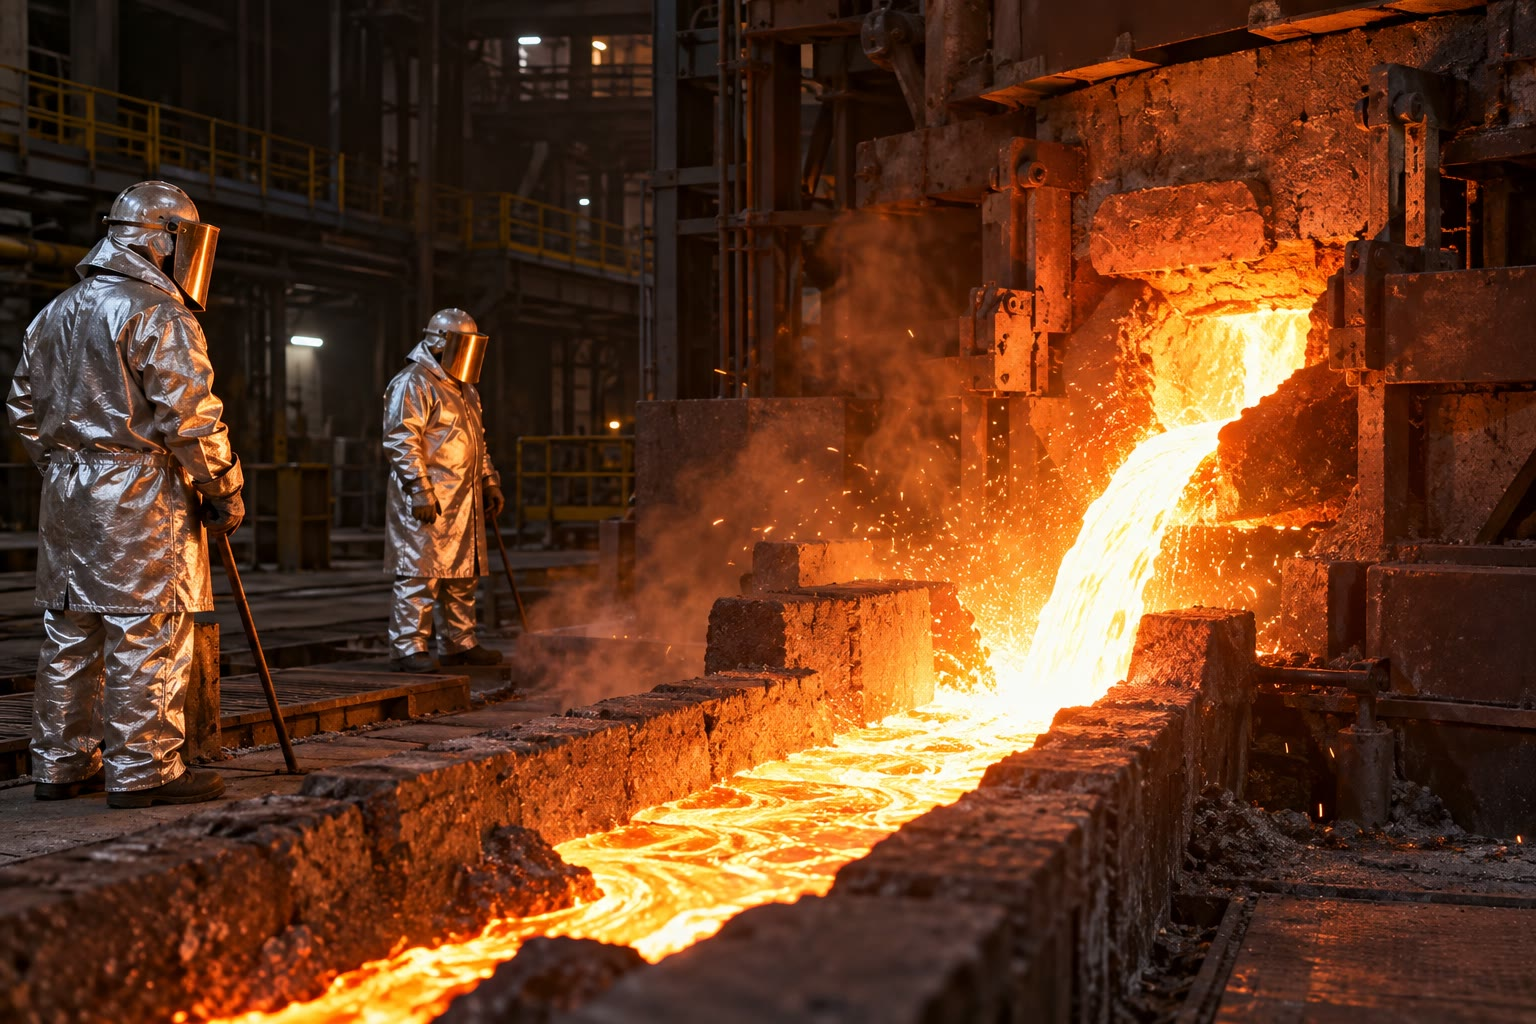
\includegraphics[width=0.62\linewidth]{images/book3/ai/b2-06-blast-furnace.jpg}

{\small वात्या भट्ठी से निकासी: द्रव लोहा एक दुर्गलनीय नाली में बहता है,
जिसे ऊष्मा-परावर्ती पोशाक पहने श्रमिक देख रहे हैं। भट्ठी के भीतर का ताप और
गैस वही हैं जो कार्बन मोनॉक्साइड को आयरन ऑक्साइड से ऑक्सीजन
छीनने देते हैं।}
\end{omfigure}

\section{एलिंगम आरेख}

भिन्न धातुओं की ऑक्सीजन के प्रति बंधुता की तुलना करने के लिए अभिक्रियाएँ
इस प्रकार लिखी जाती हैं कि सभी समान अभिकर्मक की समान मात्रा का उपभोग करें।

\begin{definition}[एलिंगम आरेख]\label{def:b2:ellingham:diagram}
ऑक्साइडों के किसी परिवार का \emph{एलिंगम आरेख}\index{एलिंगम आरेख}
डाइऑक्सीजन के एक मोल के लिए लिखी गई उनकी संभवन अभिक्रियाओं की मानक गिब्स
ऊर्जाओं का ताप के सापेक्ष आलेख है,
\[
  \tfrac{2x}{y}\,\mathrm M + \ce{O2} \longrightarrow \tfrac{2}{y}\,\mathrm{M}_x\mathrm O_y ,
  \qquad \Delta_r G^\circ(T) \ \text{प्रति मोल } \ce{O2} .
\]
\end{definition}

उदाहरण के लिए \ce{2Zn + O2 -> 2ZnO}, \ce{4/3Al + O2 -> 2/3Al2O3}, \ce{2C + O2 ->
2CO}। कोटि-अक्ष \unit{kJ} प्रति मोल \ce{O2} में है, जो चार्ट की
धातुओं के लिए सदा ऋणात्मक है।

\begin{proposition}[सरल रेखाएँ]\label{prop:b2:ellingham:line}
\omterm{def:b2:reaction-free-energy:ellingham-approximation}{एलिंगम सन्निकटन} में हर रेखा सरल है, जिसकी प्रवणता $-\Delta_r
S^\circ$ है। किसी धातु और उसके ऑक्साइड के लिए, दोनों संघनित होने पर, $\Delta_r S^\circ$
उपभुक्त डाइऑक्सीजन के मोल की एन्ट्रॉपी के ऋण के निकट होता है, लगभग
$-\qty{200}{J/(K.mol)}$: रेखाएँ ताप के साथ ऊपर उठती हैं, सभी लगभग
समान प्रवणता से।
\end{proposition}

\begin{proof}
$\Delta_r G^\circ = \Delta_r H^\circ - T\Delta_r S^\circ$, स्थिर $\Delta_r
H^\circ$, $\Delta_r S^\circ$ के साथ। ठोसों की मोलर एन्ट्रॉपियाँ दसियों
\unit{J/(K.mol)} होती हैं और धातु तथा ऑक्साइड के बीच बड़े अंश में कट जाती हैं, जबकि
गैस का एक मोल उपभुक्त होता है, जिसकी एन्ट्रॉपी $S^\circ(\ce{O2}) = \qty{205}{J/(K.mol)}$ है। ज़िंक के लिए
$2(43.65) - 2(41.63) - 205.15 = \qty{-201.1}{J/(K.mol)}$।
% ledger: s0:ZnO_cr, s0:Zn_cr, s0:O2_g
\end{proof}

\begin{proposition}[रेखाओं में मोड़]\label{prop:b2:ellingham:break}
जिस ताप पर धातु पिघलती या उबलती है, वहाँ रेखा की प्रवणता बदल जाती है:
उसकी प्रवणता $\nu\,\Delta_{\text{संक्रमण}}S$ से बढ़ती है, जहाँ $\nu$ अभिक्रिया में
धातु की मात्रा है और $\Delta_{\text{संक्रमण}}S = \Delta_{\text{संक्रमण}}H/T_{\text{संक्रमण}}$।
इसके विपरीत, ऑक्साइड का अवस्था-परिवर्तन प्रवणता को घटाता है।
\end{proposition}

\begin{proof}
संक्रमण से ऊपर धातु अपनी नई प्रावस्था से अभिक्रिया करती है, जिसकी एन्ट्रॉपी
$\Delta_{\text{संक्रमण}}S$ अधिक है: $\Delta_r S^\circ$, $\nu\,\Delta_{\text{संक्रमण}}S$ से घटता है
और प्रवणता $-\Delta_r S^\circ$ उतनी ही बढ़ती है। $\Delta_r G^\circ$
स्वयं संतत है, क्योंकि $T_{\text{संक्रमण}}$ पर दोनों प्रावस्थाओं का
\omterm{def:b2:chemical-potential:chemical-potential}{रासायनिक विभव} समान है। ऑक्साइड के लिए विपरीत चिह्न।
\end{proof}

गलन प्रवणता को थोड़ा बदलता है; क्वथन, जो किसी संघनित अभिकारक को
गैस बना देता है, बहुत। ज़िंक \qty{1180}{K} पर उबलता है: उस ताप से ऊपर
ज़िंक ऑक्साइड का संभवन ऑक्साइड के प्रति दो मोल पर गैस के तीन मोल उपभुक्त करता है,
और उसकी रेखा तीव्रता से ऊपर चढ़ती है। मैग्नीशियम के साथ भी उसके क्वथनांक से
ऊपर यही होता है।

\begin{omfigure}
\begin{tikzpicture}[lab/.style={anchor=west, font=\scriptsize, inner sep=1pt}]
\begin{axis}[omellingham,
  width=0.84\linewidth, height=11cm, xmin=300, xmax=2100, ymin=-1250, ymax=0,
  clip mode=individual,
  xlabel={$T$ (K)}, ylabel={$\Delta_r G^\circ$ (\unit{kJ} प्रति mol \ce{O2})},
  xtick={300,500,700,900,1100,1300,1500,1700,1900,2100},
  x tick label style={rotate=45, anchor=north east, font=\scriptsize}]
\addplot[black!60, thick] table[x=T, y=G] {figdata/out/bachelor-2-ellingham-a-HgO.dat};
\addplot[omProp, thick] table[x=T, y=G] {figdata/out/bachelor-2-ellingham-a-Cu2O.dat};
\addplot[omDef, thick] table[x=T, y=G] {figdata/out/bachelor-2-ellingham-a-FeO.dat};
\addplot[omExo, very thick] table[x=T, y=G] {figdata/out/bachelor-2-ellingham-a-ZnO.dat};
\addplot[black!60, thick] table[x=T, y=G] {figdata/out/bachelor-2-ellingham-a-Cr2O3.dat};
\addplot[omProp, thick] table[x=T, y=G] {figdata/out/bachelor-2-ellingham-a-TiO2.dat};
\addplot[omDef, thick] table[x=T, y=G] {figdata/out/bachelor-2-ellingham-a-Al2O3.dat};
\addplot[black!60, thick] table[x=T, y=G] {figdata/out/bachelor-2-ellingham-a-MgO.dat};
\addplot[omProp, thick] table[x=T, y=G] {figdata/out/bachelor-2-ellingham-a-CaO.dat};
\addplot[omThm, very thick] table[x=T, y=G] {figdata/out/bachelor-2-ellingham-a-C-CO.dat};
\addplot[omThm, thick, dashed] table[x=T, y=G] {figdata/out/bachelor-2-ellingham-a-C-CO2.dat};
\addplot[omThm, thick, dotted] table[x=T, y=G] {figdata/out/bachelor-2-ellingham-a-CO-CO2.dat};
\addplot[omDef, thick, dashed] table[x=T, y=G] {figdata/out/bachelor-2-ellingham-a-H2-H2O.dat};
% labels: inside for the two short lines, at the right end for the others
\node[font=\scriptsize, black!70, anchor=south] at (axis cs:400,-60) {\ce{HgO}};
\node[font=\scriptsize, omProp, anchor=south] at (axis cs:1100,-150) {\ce{Cu2O}};
\draw[omExo, thin] (axis cs:2100,-69) -- (axis cs:2150,-60) node[lab, text=omExo] {\ce{ZnO}};
\draw[omThm, thin] (axis cs:2100,-204) -- (axis cs:2150,-185) node[lab, text=omThm] {\ce{CO}/\ce{CO2}};
\draw[omDef, thin] (axis cs:2100,-259) -- (axis cs:2150,-235) node[lab, text=omDef] {\ce{H2}/\ce{H2O}};
\draw[omDef, thin] (axis cs:2100,-286) -- (axis cs:2150,-285) node[lab, text=omDef] {\ce{FeO}};
\draw[black!70, thin] (axis cs:2100,-393) -- (axis cs:2150,-365) node[lab, text=black!70] {\ce{Cr2O3}};
\draw[omThm, thin] (axis cs:2100,-396) -- (axis cs:2150,-415) node[lab, text=omThm] {\ce{C}/\ce{CO2}};
\draw[omProp, thin] (axis cs:2100,-567) -- (axis cs:2150,-540) node[lab, text=omProp] {\ce{TiO2}};
\draw[omThm, thin] (axis cs:2100,-589) -- (axis cs:2150,-590) node[lab, text=omThm] {\ce{C}/\ce{CO}};
\draw[black!70, thin] (axis cs:2100,-600) -- (axis cs:2150,-640) node[lab, text=black!70] {\ce{MgO}};
\draw[omDef, thin] (axis cs:2100,-668) -- (axis cs:2150,-690) node[lab, text=omDef] {\ce{Al2O3}};
\draw[omProp, thin] (axis cs:2100,-765) -- (axis cs:2150,-765) node[lab, text=omProp] {\ce{CaO}};
\end{axis}
\end{tikzpicture}

{\small \omterm{def:b2:ellingham:diagram}{एलिंगम आरेख}: ताप के सापेक्ष प्रति मोल \ce{O2} ऑक्साइडों के संभवन की मानक
\omterm{def:b2:reaction-free-energy:gibbs-energy}{गिब्स ऊर्जा}, सारणीबद्ध गिब्स ऊर्जाओं से। जितनी नीची
रेखा, ऑक्साइड उतना अधिक स्थायी और धातु उतनी अधिक अपचायक।
हर धातु-रेखा पर उसके ऑक्साइड का नाम अंकित है; \ce{C}/\ce{CO} का अर्थ \ce{2C + O2 -> 2CO} है,
\ce{C}/\ce{CO2} का \ce{C + O2 -> CO2}, \ce{CO}/\ce{CO2} का \ce{2CO + O2 -> 2CO2}
और \ce{H2}/\ce{H2O} का \ce{2H2 + O2 -> 2H2O}, जल गैस के रूप में।}
% ledger: janafG:Cu2O.300, janafG:FeO.300, janafG:Cr2O3.300, janafG:TiO2.500, janafG:Al2O3.300, janafG:MgO.300, janafG:CaO.300, janafG:CO.300, janafG:CO2.300, janafG:H2O.300, dfh:ZnO_cr, dfh:HgO_cr, s0:HgO_cr, s0:Hg_l, s0:Hg_g, dfh:Hg_g (all temperatures in figdata/bachelor-2/ellingham.py)
\end{omfigure}

\section{आरेख को पढ़ना}

\begin{definition}[साम्य ऑक्सीजन दाब]\label{def:b2:ellingham:oxygen-pressure}
ताप $T$ पर किसी धातु–ऑक्साइड युग्म का \emph{साम्य ऑक्सीजन दाब}\index{साम्य ऑक्सीजन दाब}
डाइऑक्सीजन का वह दाब है जिस पर धातु
और ऑक्साइड साम्य में सह-अस्तित्व रखते हैं: प्रति मोल \ce{O2} लिखी गई अभिक्रिया के लिए
$RT\ln(p_{\ce{O2}}/p^\circ) = \Delta_r
G^\circ(T)$।
\end{definition}

\begin{theorem}[धातु और ऑक्साइड के क्षेत्र]\label{thm:b2:ellingham:domains}
ऑक्सीजन दाब $p_{\ce{O2}}$ वाले वायुमंडल में, ताप $T$ पर,
धातु ऑक्सीकृत होती है यदि $RT\ln(p_{\ce{O2}}/p^\circ) > \Delta_r G^\circ(T)$, और
ऑक्साइड धातु में अपचित होता है यदि $RT\ln(p_{\ce{O2}}/p^\circ) < \Delta_r
G^\circ(T)$। आरेख पर ऑक्साइड अपनी रेखा के ऊपर स्थायी है, धातु
नीचे।
\end{theorem}

\begin{proof}
सक्रियता 1 वाले संघनित धातु और ऑक्साइड के साथ $Q = p^\circ/p_{\ce{O2}}$ और
$\Delta_r G = \Delta_r G^\circ + RT\ln Q = \Delta_r G^\circ - RT\ln(p_{\ce{O2}}/
p^\circ)$। ऑक्सीकरण अग्र दिशा में चलता है जब $\Delta_r G < 0$।
\end{proof}

वायु में ($p_{\ce{O2}} = \qty{0.21}{bar}$, $RT\ln 0.21$ कमरे के ताप पर \qty{-4}{kJ/mol}
और \qty{1000}{K} पर \qty{-13}{kJ/mol} है, इस पैमाने पर लगभग
शून्य) आरेख की हर वह धातु जिसकी रेखा अक्ष के नीचे है
ऑक्सीकृत होती है: कमरे के ताप पर सभी, ताँबा भी। केवल
ऊपर के निकट के ऑक्साइड (चाँदी, पारा) मध्यम तापन पर
विघटित होते हैं।

\begin{example}[पारे का ऑक्साइड]\label{ex:b2:ellingham:hgo}
\ce{2Hg + O2 -> 2HgO} के लिए CODATA के मुख्य मान द्रव पारे के साथ $\Delta_r H^\circ =
\qty{-181.6}{kJ/mol}$ देते हैं; पारे के क्वथनांक से ऊपर
धातु गैस है और $\Delta_r H^\circ = \qty{-304.3}{kJ/mol}$, $\Delta_r
S^\circ = \qty{-414.6}{J/(K.mol)}$। रेखा शून्य को
$T = 304.3/0.4146 \approx \qty{734}{K}$ पर काटती है: वायु में,
या \qty{1}{bar} ऑक्सीजन के अंतर्गत, उस ताप से ऊपर गर्म करने पर लाल मर्क्यूरिक ऑक्साइड अपनी ऑक्सीजन छोड़ देता है ---
इसी प्रकार 1774 में ऑक्सीजन पहली बार पृथक की गई थी।
% ledger: dfh:HgO_cr, s0:HgO_cr, s0:Hg_l, s0:Hg_g, dfh:Hg_g, s0:O2_g (computed in figdata/bachelor-2/ellingham.py)
\end{example}

\begin{proposition}[कौन-सी धातु किस ऑक्साइड का अपचयन करती है]\label{prop:b2:ellingham:reduction}
दिए गए ताप पर, मानक परिस्थितियों में, धातु M धातु N के ऑक्साइड का अपचयन करती है
जब M की रेखा N की रेखा से नीचे हो। अपचयन की \omterm{def:b2:reaction-free-energy:reaction-gibbs}{मानक
अभिक्रिया गिब्स ऊर्जा}, स्थानांतरित \ce{O2} के प्रति मोल, दोनों
कोटियों का अंतर है।
\end{proposition}

\begin{proof}
अपचयन M के ऑक्साइड का संभवन ऋण N के ऑक्साइड का संभवन है, दोनों प्रति
मोल \ce{O2}: $\Delta_r G^\circ = \Delta_r G^\circ_{\mathrm M} - \Delta_r
G^\circ_{\mathrm N}$, जो ऋणात्मक है जब M की रेखा नीची हो।
\end{proof}

\begin{method}[एलिंगम आरेख पढ़ना]\label{met:b2:ellingham:read-ellingham}
\begin{enumerate}
  \item वांछित ताप पर दोनों रेखाएँ खोजिए। नीची रेखा
        अधिक स्थायी ऑक्साइड की है; उसकी धातु दूसरे ऑक्साइड का अपचयन करती है।
  \item ऊर्ध्वाधर अंतराल प्रति मोल \ce{O2} $\Delta_r G^\circ$ है:
        \qty{100}{kJ} या उससे अधिक का अंतराल व्यवहार में पूर्ण अपचयन का अर्थ रखता है।
  \item जहाँ दो रेखाएँ एक-दूसरे को काटती हैं, वहाँ अपचयन की दिशा बदल जाती है:
        प्रतिच्छेद का ताप पढ़िए।
  \item मोड़ों पर ध्यान दीजिए: अंतराल के भीतर उबलने वाली धातु
        वाष्प के रूप में निकलती है, जिसे आसवित करके अलग किया जा सकता है --- या जो ठंडा होने पर फिर ऑक्सीकृत हो जाती है।
\end{enumerate}
\end{method}

\begin{definition}[ऐलुमिनोतापी अपचयन]\label{def:b2:ellingham:aluminothermy}
\emph{ऐलुमिनोतापी अपचयन}\index{ऐलुमिनोतापी अपचयन} किसी धातु ऑक्साइड का
ऐलुमिनियम चूर्ण द्वारा अपचयन है, जो हर उस ऑक्साइड के लिए संभव है जिसकी
रेखा ऐलुमिना की रेखा से ऊपर है, और इतना \omterm{def:b2:reaction-enthalpy:exothermic}{ऊष्माक्षेपी} कि मिश्रण पिघल जाता है:
\ce{Fe2O3 + 2Al -> Al2O3 + 2Fe} (थर्माइट) रेलों को जोड़ता है; \ce{Cr2O3 + 2Al ->
Al2O3 + 2Cr} कार्बन-रहित क्रोमियम बनाता है।
\end{definition}

\begin{omfigure}
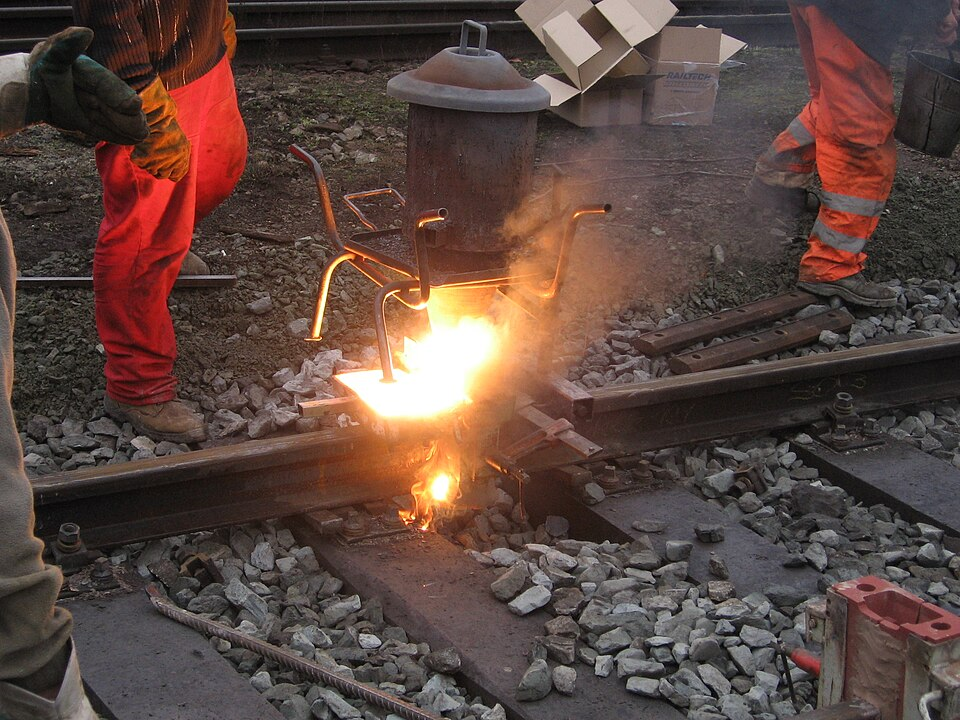
\includegraphics[width=0.5\linewidth]{images/book3/thermite.jpg}

{\small एक रेल की थर्माइट वेल्डिंग: जोड़ के ऊपर कुठाली में आयरन ऑक्साइड की
ऐलुमिनियम से अभिक्रिया द्रव लोहा देती है, जो दोनों रेल-सिरों के बीच के
साँचे में नीचे बहता है। (छायाचित्र: पेत्र एस॰, CC BY-SA 3.0, विकिमीडिया
कॉमन्स।)}
\end{omfigure}

\section{कार्बन और कार्बन मोनॉक्साइड}

तीन रेखाओं में कार्बन सम्मिलित है:
\begin{itemize}
  \item \ce{C + O2 -> CO2}: गैस का एक मोल एक देता है, $\Delta_r S^\circ
        \approx 0$, \qty{-395}{kJ} के निकट लगभग क्षैतिज रेखा;
  \item \ce{2C + O2 -> 2CO}: गैस का एक मोल दो देता है, $\Delta_r S^\circ
        \approx \qty{+180}{J/(K.mol)}$, ऐसी रेखा जो ताप के साथ \emph{गिरती} है;
  \item \ce{2CO + O2 -> 2CO2}: गैस के तीन मोल दो देते हैं, एक चढ़ती रेखा।
\end{itemize}

\begin{proposition}[गर्म होने पर कार्बन लगभग हर चीज़ का अपचयन करता है]\label{prop:b2:ellingham:carbon}
\ce{2C + O2 -> 2CO} की रेखा ताप के साथ घटती है और अधिकांश धातु ऑक्साइडों की
रेखाओं को काटती है: प्रतिच्छेद ताप से ऊपर कार्बन ऑक्साइड का अपचयन करता है
और कार्बन मोनॉक्साइड देता है। आयरन(II) ऑक्साइड के लिए प्रतिच्छेद लगभग
\qty{1040}{K} पर है, ज़िंक ऑक्साइड के लिए लगभग \qty{1220}{K} पर; टाइटेनिया और मैग्नीशिया के लिए
यह \qty{2000}{K} के निकट या उससे ऊपर है, ऐलुमिना के लिए और भी ऊँचा, जहाँ धातुएँ
कार्बन के साथ कार्बाइड बनाती हैं या गैस के ठंडा होने पर फिर ऑक्सीकृत हो जाती हैं।
\end{proposition}

\begin{proof}
कार्बन रेखा की प्रवणता $-\Delta_r S^\circ$ ऋणात्मक है ($\Delta\nu_{\text{गैस}}
= +1$), ऑक्साइड रेखाओं की धनात्मक: वे एक बार मिलती हैं। ताप
परिकलित रेखाओं पर पढ़े जाते हैं।
% ledger: janafG:CO.900, janafG:CO.1100, janafG:FeO.900, janafG:FeO.1100 (crossings computed in figdata/bachelor-2/ellingham.py)
\end{proof}

\begin{definition}[बूदुआर साम्य]\label{def:b2:ellingham:boudouard}
\emph{बूदुआर साम्य}\index{बूदुआर साम्य} \ce{C(s) + CO2(g) <=> 2CO(g)} है,
\omterm{def:b2:reaction-enthalpy:exothermic}{ऊष्माशोषी}, कार्बन और कार्बन के दो ऑक्साइडों के बीच।
\end{definition}

\begin{proposition}[कार्बन के ऊपर गैस का संघटन]\label{prop:b2:ellingham:boudouard}
निकाय कार्बन + \ce{CO} + \ce{CO2} की \omterm{def:b2:equilibrium-shifts:variance}{स्वातंत्र्य कोटि} 2 है: दिए गए $T$ और कुल
दाब $p$ पर कार्बन मोनॉक्साइड का मोल अंश $x$, $x^2/(1 - x)
= K^\circ(T)\,p^\circ/p$ द्वारा नियत होता है। \qty{1}{bar} पर गैस \qty{700}{K} से नीचे लगभग शुद्ध \ce{CO2}
और \qty{1200}{K} से ऊपर लगभग शुद्ध \ce{CO} होती है; तीनों कार्बन
रेखाओं का प्रतिच्छेद, लगभग \qty{975}{K} पर, वहाँ है जहाँ $K^\circ = 1$।
\end{proposition}

\begin{proof}
तीन स्पीशीज़, एक अभिक्रिया, दो प्रावस्थाएँ: $v = 3 - 1 + 2 - 2 = 2$। $p_{\ce{CO}}
= xp$ और $p_{\ce{CO2}} = (1 - x)p$ के साथ $Q = x^2p/[(1 - x)p^\circ]$। $K^\circ = 1$ पर
\ce{2C + O2 -> 2CO} और \ce{C + O2 -> CO2} की मानक गिब्स ऊर्जाएँ
बराबर होती हैं: दोनों रेखाएँ, और इसलिए तीसरी भी, मिलती हैं।
\end{proof}

\begin{omfigure}
\begin{tikzpicture}
\begin{axis}[
  width=0.62\linewidth, height=5.4cm, xmin=500, xmax=1500, ymin=0, ymax=1.05,
  axis x line=bottom, axis y line=left, xlabel={$T$ (K)},
  xtick={500,700,900,1100,1300,1500}, ytick={0,0.5,1},
  ylabel={\ce{CO} का मोल अंश}, tick label style={font=\small},
  label style={font=\small}, clip=false]
\addplot[omThm, very thick] table[x=T, y=xCO] {figdata/out/bachelor-2-ellingham-b.dat};
\node[font=\scriptsize, anchor=west] at (axis cs:1150,0.55) {\ce{CO} स्थायी};
\node[font=\scriptsize, anchor=west] at (axis cs:510,0.6) {\ce{CO2} (और कार्बन) स्थायी};
\end{axis}
\end{tikzpicture}

{\small \qty{1}{bar} पर \omterm{def:b2:ellingham:boudouard}{बूदुआर साम्य}: कार्बन के साथ साम्य में गैस में कार्बन
मोनॉक्साइड का मोल अंश।}
% ledger: janafG:CO.700, janafG:CO2.700, janafG:CO.1100, janafG:CO2.1100 (computed in figdata/bachelor-2/ellingham.py)
\end{omfigure}

\section{वात्या भट्ठी}

लौह अयस्क (हेमाटाइट \ce{Fe2O3}, मैग्नेटाइट \ce{Fe3O4}), कोक और चूना पत्थर
एक ऊँचे स्तंभ के शीर्ष पर भरे जाते हैं; तली के निकट गर्म वायु
फूँकी जाती है। नीचे उतरते हुए ठोस ऊपर उठती गर्म गैस से मिलते हैं; गैस
ठंडी होकर शीर्ष से निकलती है।
\begin{itemize}
  \item टुयरे पर कोक गर्म वायु में जलता है: \ce{C + O2 -> CO2}, और
        उसके ऊपर, अधिक कार्बन के साथ, \ce{CO2 + C -> 2CO} (बूदुआर): ऊपर उठने वाली
        गैस मुख्यतः कार्बन मोनॉक्साइड और नाइट्रोजन होती है।
  \item ऊपरी भाग में कार्बन मोनॉक्साइड आयरन ऑक्साइडों का चरण-दर-चरण
        अपचयन करती है, \ce{3Fe2O3 + CO -> 2Fe3O4 + CO2}, \ce{Fe3O4 + CO -> 3FeO + CO2},
        \ce{FeO + CO -> Fe + CO2}। पहले दो चरण आसान हैं; अंतिम के लिए
        \ce{CO}/\ce{CO2} रेखा \ce{FeO} की रेखा से थोड़ा \textit{ऊपर}
        चलती है: उसकी \omterm{def:b2:reaction-free-energy:reaction-gibbs}{मानक अभिक्रिया गिब्स ऊर्जा} थोड़ी धनात्मक है
        (\qty{900}{K} पर $K^\circ \approx 0.3$), और अपचयन के लिए ऐसी गैस चाहिए
        जिसमें \ce{CO} की मात्रा \ce{CO2} से कम से कम तीन गुना हो --- जिसे नीचे के गर्म क्षेत्र में
        \omterm{def:b2:ellingham:boudouard}{बूदुआर साम्य} प्रदान करता है।
  \item नीचे और अधिक गर्म भाग में कार्बन स्वयं बचे हुए का अपचयन करता है, \ce{FeO + C ->
        Fe + CO}; लोहा कार्बन घोलता है, पिघलता है, और तली में
        अयस्क की सिलिका और चूने से बने पिघले धातुमल के साथ जमा होता है।
\end{itemize}

\begin{omfigure}
\begin{tikzpicture}[font=\small, >={Stealth}]
  \fill[gray!12] (-1.4,0) -- (-2.0,3.0) -- (-1.3,7.0) -- (1.3,7.0) -- (2.0,3.0) -- (1.4,0) -- cycle;
  \draw[thick] (-1.4,0) -- (-2.0,3.0) -- (-1.3,7.0) (1.4,0) -- (2.0,3.0) -- (1.3,7.0);
  \draw[thick] (-1.4,0) -- (1.4,0);
  \fill[orange!70!red] (-1.4,0) rectangle (1.4,0.35);
  \fill[yellow!50!orange] (-1.45,0.35) rectangle (1.45,0.6);
  \node[font=\scriptsize] at (0,0.17) {द्रव लोहा};
  \node[font=\scriptsize] at (0,0.48) {धातुमल};
  % tuyeres
  \draw[->, thick, omDef] (-3.2,1.2) -- (-1.75,1.2) node[pos=0, left] {गर्म वायु};
  \draw[->, thick, omDef] (3.2,1.2) -- (1.75,1.2);
  % charge and gas
  \draw[->, thick] (-0.6,7.9) -- (-0.6,7.1) node[pos=0, above left, xshift=6pt] {अयस्क, कोक, चूना पत्थर};
  \draw[->, thick, omThm] (0.7,7.1) -- (0.7,7.9) node[pos=1, above right, xshift=-6pt] {शीर्ष गैस (\ce{CO}, \ce{CO2}, \ce{N2})};
  \draw[->, omThm, thick] (0.6,1.6) -- (0.6,6.4);
  \draw[->, thick] (-0.6,6.4) -- (-0.6,1.6);
  \node[omThm, font=\scriptsize, rotate=90] at (0.9,4.0) {गैस ऊपर उठती है};
  \node[font=\scriptsize, rotate=90] at (-0.9,4.0) {ठोस नीचे उतरते हैं};
  % zones
  \node[anchor=west, align=left, font=\scriptsize] at (2.3,6.0) {\ce{3Fe2O3 + CO -> 2Fe3O4 + CO2}\\ \ce{Fe3O4 + CO -> 3FeO + CO2}};
  \node[anchor=west, align=left, font=\scriptsize] at (2.3,4.2) {\ce{FeO + CO -> Fe + CO2}};
  \node[anchor=west, align=left, font=\scriptsize] at (2.3,2.7) {\ce{CO2 + C -> 2CO}\\ \ce{FeO + C -> Fe + CO}};
  \node[anchor=west, align=left, font=\scriptsize] at (2.3,1.6) {\ce{C + O2 -> CO2}};
  \draw[densely dotted] (1.95,6.0) -- (2.3,6.0) (1.9,4.2) -- (2.3,4.2) (2.0,2.8) -- (2.3,2.8);
  \node[anchor=east, align=right, font=\scriptsize, black!60] at (-2.2,6.0) {ठंडा};
  \node[anchor=east, align=right, font=\scriptsize, black!60] at (-2.2,2.3) {अधिक गर्म};
  \draw[->, black!50] (-2.6,5.6) -- (-2.6,2.7);
\end{tikzpicture}

{\small प्रतिधारा रिएक्टर के रूप में वात्या भट्ठी। ठोस नीचे जाते हैं, गर्म
अपचायक गैस ऊपर जाती है; आयरन ऑक्साइडों का अपचयन ऊपरी, ठंडे भाग में कार्बन
मोनॉक्साइड द्वारा, और निचले, अधिक गर्म भाग में कार्बन द्वारा होता है। लोहा और धातुमल
तली से निकाले जाते हैं।}
\end{omfigure}

\begin{omfigure}
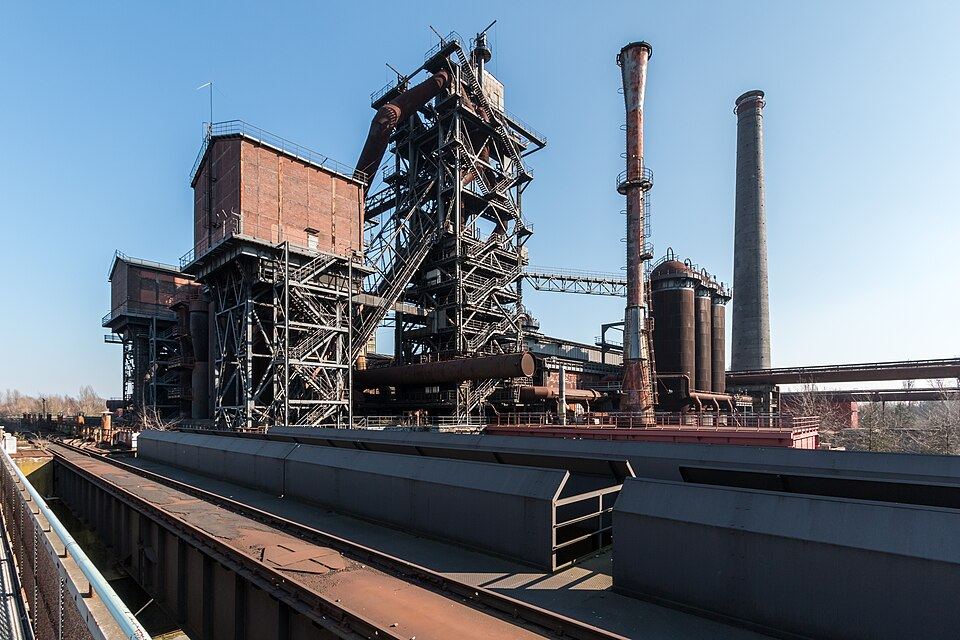
\includegraphics[width=0.6\linewidth]{images/book3/blast-furnace.jpg}

{\small स्मारक के रूप में संरक्षित एक वात्या भट्ठी (डुइसबर्ग-नॉर्ड, 1985 में
बंद): ऊँचा स्तंभ, गर्म वायु के पाइपों के वलय के साथ, और शीर्ष पर गैस निकास।
(छायाचित्र: डीटमार राबिख, CC BY-SA 4.0, विकिमीडिया कॉमन्स।)}
\end{omfigure}

\section{धातु तक पहुँचने के अन्य मार्ग}

\begin{definition}[ताप-धातुकर्म और जल-धातुकर्म]\label{def:b2:ellingham:metallurgy}
\emph{ताप-धातुकर्म}\index{ताप-धातुकर्म} धातु को उच्च
ताप पर, भट्ठी में उसके ऑक्साइड के अपचयन द्वारा, निष्कर्षित करता है। \emph{जल-धातुकर्म}\index{जल-धातुकर्म}
उसे जलीय विलयन से निष्कर्षित करता है। इनके सामान्य चरण हैं:
\emph{भर्जन}\index{भर्जन} (सल्फ़ाइड अयस्क को वायु में गर्म करके उसे
ऑक्साइड में बदलना, \ce{2ZnS + 3O2 -> 2ZnO + 2SO2}), \emph{निक्षालन}\index{निक्षालन}
(धातु के यौगिक को, प्रायः सल्फ़्यूरिक अम्ल में, घोलना, \ce{ZnO + 2H+ ->
Zn^2+ + H2O}), विलयन का शोधन, उदाहरण के लिए
\emph{सीमेंटीकरण}\index{सीमेंटीकरण} द्वारा (कम उत्कृष्ट धातु के चूर्ण द्वारा
अधिक उत्कृष्ट धातु के आयनों का अपचयन, \ce{Cu^2+ + Zn -> Cu + Zn^2+}), और
धातु की पुनःप्राप्ति, प्रायः विद्युत-अपघटन द्वारा।
\end{definition}

आरेख श्रम-विभाजन को समझाता है। लोहा, ज़िंक, सीसा, टिन भट्ठी में
कार्बन द्वारा प्राप्त किए जाते हैं। ऐलुमिनियम, जिसकी रेखा किसी भी व्यावहारिक ताप पर कार्बन की
रेखा से बहुत नीचे है, अपने पिघले ऑक्साइड के विद्युत-अपघटन से बनता है
(\cref{ch:b2:batteries-electrolysis}); मैग्नीशियम विद्युत-अपघटन से या
निर्वात में सिलिकॉन द्वारा अपचयन से, जो मैग्नीशियम वाष्प को हटा देता है;
टाइटेनियम ऑक्साइड को क्लोराइड में बदलकर, \ce{TiO2 + 2Cl2 + C -> TiCl4 +
CO2} (\cref{exo:b2:reaction-free-energy:12}), फिर क्लोराइड का
मैग्नीशियम से अपचयन करके (क्रोल प्रक्रम)। संसार का अधिकांश ज़िंक \omterm{def:b2:ellingham:metallurgy}{भर्जन},
\omterm{def:b2:ellingham:metallurgy}{निक्षालन} और विद्युत-अपघटन से बनता है: जल-धातुकर्मी मार्ग अधिक शुद्ध धातु देता है और
ज़िंक वाष्प से निपटने से बचाता है।

\begin{omfigure}
\begin{tikzpicture}[font=\small, >={Stealth}, box/.style={draw, thick, rounded corners=2pt, align=center, minimum height=0.9cm, fill=white, text width=2.3cm}]
  \node[box] (r) at (0,0) {भर्जन\\ \ce{ZnS} $\to$ \ce{ZnO}};
  \node[box] (l) at (3.2,0) {\ce{H2SO4} में\\ निक्षालन};
  \node[box] (c) at (6.4,0) {शोधन\\ (सीमेंटीकरण)};
  \node[box] (e) at (9.6,0) {विद्युत-अपघटन\\ \ce{Zn^2+} $\to$ \ce{Zn}};
  \draw[->, thick] (r) -- (l); \draw[->, thick] (l) -- (c); \draw[->, thick] (c) -- (e);
  \draw[->, thick, black!60] (r.north) -- ++(0,0.7) node[above] {\ce{SO2} $\to$ सल्फ़्यूरिक अम्ल};
  \draw[->, thick, omThm] (e.south) -- ++(0,-0.6) -| (l.south) node[pos=0.25, below] {लौटाया गया अम्ल};
  \draw[->, thick] (e.east) -- ++(0.8,0) node[right] {ज़िंक};
\end{tikzpicture}

{\small ज़िंक तक जल-धातुकर्मी मार्ग। भर्जक की सल्फ़र डाइऑक्साइड से
\omterm{def:b2:ellingham:metallurgy}{निक्षालन} का सल्फ़्यूरिक अम्ल बनाया जाता है; विद्युत-अपघटन के
ऐनोड पर पुनर्जनित अम्ल उसी में लौटा दिया जाता है।}
\end{omfigure}

\section{अभ्यास}

\begin{exercise}[$\star$]\label{exo:b2:ellingham:1}
कॉपर(I) ऑक्साइड, ऐलुमिना, कार्बन मोनॉक्साइड और कार्बन डाइऑक्साइड की रेखाओं द्वारा
निरूपित अभिक्रियाएँ लिखिए, हर एक \ce{O2} के एक मोल के लिए।
\end{exercise}

\begin{exercise}[$\star$]\label{exo:b2:ellingham:2}
CODATA के मुख्य मानों ($\Delta_f H^\circ(\ce{ZnO}) = \qty{-350.46}{kJ/mol}$,
$S^\circ$: \ce{ZnO} 43.65, \ce{Zn} 41.63, \ce{O2} \qty{205.15}{J/(K.mol)}) से
ठोस ज़िंक के लिए \ce{2Zn + O2 -> 2ZnO} का $\Delta_r G^\circ(T)$ लिखिए।
\end{exercise}

\begin{exercise}[$\star$]\label{exo:b2:ellingham:3}
आरेख से वे धातुएँ सूचीबद्ध कीजिए जो \qty{1500}{K} पर क्रोमियम(III) ऑक्साइड का
अपचयन कर सकती हैं, और वे जो नहीं कर सकतीं।
\end{exercise}

\begin{exercise}[$\star$]\label{exo:b2:ellingham:4}
तीनों कार्बन रेखाओं में से हर एक की प्रवणता का चिह्न समझाइए।
\end{exercise}

\begin{exercise}[$\star\star$]\label{exo:b2:ellingham:5}
\qty{600}{K} पर मर्क्यूरी(II) ऑक्साइड का \omterm{def:b2:ellingham:oxygen-pressure}{साम्य ऑक्सीजन दाब} परिकलित कीजिए
(पारा द्रव, $\Delta_r H^\circ = \qty{-181.6}{kJ}$, $\Delta_r S^\circ =
\qty{-216.5}{J/K}$ प्रति मोल \ce{O2})। क्या उस ताप पर पारा वायु में
ऑक्सीकृत होता है?
\end{exercise}

\begin{exercise}[$\star\star$]\label{exo:b2:ellingham:6}
थर्माइट अभिक्रिया, \ce{Fe2O3 +
2Al -> Al2O3 + 2Fe}, का \qty{298}{K} पर $\Delta_r G^\circ$ परिकलित कीजिए, जबकि
\ce{Fe2O3} के लिए $\Delta_f G^\circ = \qty{-743.5}{kJ/mol}$ और \ce{Al2O3} के लिए \qty{-1582.3}{kJ/mol}
दिए हैं, और बताइए कि अत्यंत \omterm{def:b2:reaction-free-energy:exergonic}{ऊर्जामोची} होते हुए भी अभिक्रिया
कमरे के ताप पर आरंभ क्यों नहीं होती।
% ledger: janafG:Fe2O3.298, janafG:Al2O3.298
\end{exercise}

\begin{exercise}[$\star\star$]\label{exo:b2:ellingham:7}
आरेख पर वह ताप खोजिए जिससे ऊपर कार्बन, कार्बन मोनॉक्साइड बनाते हुए,
आयरन(II) ऑक्साइड का लोहे में अपचयन करता है, और अभिक्रिया लिखिए।
\end{exercise}

\begin{exercise}[$\star\star$]\label{exo:b2:ellingham:8}
\qty{1100}{K} पर $\Delta_f G^\circ(\ce{CO}) = \qty{-209.1}{kJ/mol}$ और
$\Delta_f G^\circ(\ce{CO2}) = \qty{-396.0}{kJ/mol}$। \omterm{def:b2:ellingham:boudouard}{बूदुआर साम्य} का
$K^\circ$ और \qty{1}{bar} पर कार्बन के ऊपर कार्बन मोनॉक्साइड का मोल अंश परिकलित कीजिए।
कालिख या लोहे के संपर्क में गैस को \qty{700}{K} तक ठंडा करने पर
उसका क्या होता है?
% ledger: janafG:CO.1100, janafG:CO2.1100
\end{exercise}

\begin{exercise}[$\star\star$]\label{exo:b2:ellingham:9}
टंगस्टन ऑक्साइड के अपचयन के लिए कभी-कभी हाइड्रोजन प्रयुक्त होती है। जल की रेखा से
समझाइए कि उच्च ताप पर हाइड्रोजन कार्बन मोनॉक्साइड से बेहतर अपचायक है, परंतु
निम्न ताप पर बदतर।
\end{exercise}

\begin{exercise}[$\star\star\star$]\label{exo:b2:ellingham:10}
मैग्नीशियम ऑक्साइड का अपचयन सिलिकॉन द्वारा किया जा सकता है, \ce{2MgO + Si -> SiO2 + 2Mg}, यद्यपि
आरेख के हर ताप पर सिलिका की रेखा मैग्नीशिया की रेखा से ऊपर है।
\qty{1500}{K} पर मैग्नीशियम गैस है और सारणियाँ, प्रति मोल
\ce{O2}, मैग्नीशिया के लिए \qty{-845.5}{kJ} और सिलिका के लिए \qty{-643.7}{kJ} देती हैं।
अपचयन का $\Delta_r G^\circ$ परिकलित कीजिए, फिर मैग्नीशियम वाष्प का वह दाब
जिससे नीचे वह अग्र दिशा में चलता है। निर्वात भट्ठी इसका उपयोग कैसे करती है?
% ledger: janafG:MgO.1500, janafG:SiO2.1500
\end{exercise}

\begin{exercise}[$\star\star\star$]\label{exo:b2:ellingham:11}
साम्य पर निकाय \ce{FeO(s)}, \ce{Fe(s)}, \ce{CO(g)},
\ce{CO2(g)} की \omterm{def:b2:equilibrium-shifts:variance}{स्वातंत्र्य कोटि} परिकलित कीजिए। वात्या भट्ठी के ऊपरी भाग से निकलने वाली
गैस के लिए इसका क्या अर्थ है?
\end{exercise}

\begin{exercise}[$\star\star\star$]\label{exo:b2:ellingham:12}
ताँबे को उसके \omterm{def:b2:ellingham:metallurgy}{निक्षालन} विलयन से लोहे के कबाड़ द्वारा \omterm{def:b2:ellingham:metallurgy}{सीमेंटीकरण} से शुद्ध किया जाता है।
प्रथम वर्ष के खंड के मानक विभवों ($E^\circ(\ce{Cu^2+}/\ce{Cu})
= \qty{0.34}{V}$, $E^\circ(\ce{Fe^2+}/\ce{Fe}) = \qty{-0.41}{V}$) से
\ce{Cu^2+ + Fe -> Cu + Fe^2+} का साम्य स्थिरांक, और जब विलयन में \ce{Fe^2+} के
\qty{1.0}{mol/L} हों तब ताँबे के आयनों की अवशिष्ट
सांद्रता परिकलित कीजिए।
\end{exercise}

\section{समस्या: आग से ज़िंक}

\begin{problem}[{सप्ताहांत समस्या --- ज़िंक ऑक्साइड और कार्बन
मोनॉक्साइड की एलिंगम रेखाएँ, वह ताप जिस पर कार्बन ज़िंक ऑक्साइड का अपचयन करता है,
भट्ठी की स्वातंत्र्य कोटि, और ज़िंक वाष्प का संघनन}]
\label{pb:b2:ellingham:1}
विद्युत-अपघटन से पहले ज़िंक उसके ऑक्साइड को कार्बन के साथ मिट्टी के भभकों में
गर्म करके बनाया जाता था। आँकड़े (CODATA, और ज़िंक की JANAF सारणी): $\Delta_f H^\circ(\ce{ZnO})
= \qty{-350.46}{kJ/mol}$; $S^\circ$ (\unit{J/(K.mol)}): \ce{ZnO} 43.65, \ce{Zn}
41.63, \ce{O2} 205.15; ज़िंक \qty{692.7}{K} पर पिघलता है ($\Delta_{\text{गलन}}H =
\qty{7.32}{kJ/mol}$) और \qty{1}{bar} के अंतर्गत \qty{1180.2}{K} पर उबलता है
($\Delta_{\text{वाष्पन}}H = \qty{115.3}{kJ/mol}$)। \ce{2C + O2 -> 2CO} के लिए
सारणियाँ \qty{1100}{K} पर $\Delta_r G^\circ = \qty{-418.2}{kJ}$ और
\qty{1300}{K} पर \qty{-453.0}{kJ} देती हैं।
% ledger: dfh:ZnO_cr, s0:ZnO_cr, s0:Zn_cr, s0:O2_g, hT:Zn_cr.692, hT:Zn_l.692, hT:Zn_l.1180, hT:Zn_g.1180, dfh:Zn_g, janafG:CO.1100, janafG:CO.1300

\medskip
\noindent\textbf{भाग I --- ज़िंक ऑक्साइड की रेखा।}
\begin{enumerate}
  \item \qty{298}{K} पर \ce{2Zn(s) + O2 ->
        2ZnO} के $\Delta_r H^\circ$ और $\Delta_r S^\circ$ परिकलित कीजिए।
  \item गलनांक से नीचे $\Delta_r G^\circ(T)$ लिखिए।
  \item ज़िंक की गलन और वाष्पन एन्ट्रॉपियाँ परिकलित कीजिए।
  \item गलनांक और क्वथनांक के बीच $\Delta_r G^\circ(T)$ लिखिए।
  \item क्वथनांक से ऊपर इसे लिखिए।
  \item तीनों प्रवणताएँ परिकलित कीजिए और समझाइए कि अंतिम कहीं अधिक खड़ी क्यों है।
  \item जाँचिए कि संक्रमण तापों पर तीनों व्यंजक मेल खाते हैं।
\end{enumerate}

\medskip
\noindent\textbf{भाग II --- कार्बन रेखा।}
\begin{enumerate}[resume]
  \item दो सारणीबद्ध मानों से \qty{1100}{K} और \qty{1300}{K} के बीच
        \ce{2C + O2 -> 2CO} की रेखा $a + bT$ के रूप में लिखिए।
  \item इसका $\Delta_r S^\circ$ निकालिए और उसका चिह्न समझाइए।
  \item अपचयन \ce{ZnO + C -> Zn(g) + CO} और उसका $\Delta_r
        G^\circ(T)$ दोनों रेखाओं के अंतर (प्रति मोल \ce{O2}) के रूप में लिखिए।
  \item वह ताप ज्ञात कीजिए जहाँ दोनों रेखाएँ एक-दूसरे को काटती हैं।
  \item यह क्यों महत्त्वपूर्ण है कि यह ताप ज़िंक के क्वथनांक
        से ऊपर है?
\end{enumerate}

\medskip
\noindent\textbf{भाग III --- भभका।}
\begin{enumerate}[resume]
  \item निकाय \ce{ZnO(s)}, \ce{C(s)}, \ce{Zn(g)},
        \ce{CO(g)} की \omterm{def:b2:equilibrium-shifts:variance}{स्वातंत्र्य कोटि} परिकलित कीजिए, जहाँ ज़िंक और कार्बन मोनॉक्साइड केवल अपचयन से बनते हैं।
  \item \qty{1}{bar} के अंतर्गत \qty{1300}{K} पर किसी भभके में, यदि अभिक्रिया पूर्ण हो, तो ज़िंक और कार्बन
        मोनॉक्साइड के आंशिक दाब क्या हैं?
  \item \qty{1300}{K} पर अपचयन का $\Delta_r G^\circ$ और
        संगत $K^\circ$ परिकलित कीजिए।
  \item समझाइए कि भभके को प्रतिच्छेद ताप से थोड़ा ऊपर क्यों चलाया जाता है,
        उससे बहुत ऊपर क्यों नहीं।
\end{enumerate}

\medskip
\noindent\textbf{भाग IV --- संघनित्र।}
\begin{enumerate}[resume]
  \item वाष्प को एक ठंडे संघनित्र में ले जाया जाता है। वह अभिक्रिया लिखिए जिसके द्वारा
        ज़िंक वाष्प कार्बन डाइऑक्साइड द्वारा फिर ऑक्सीकृत हो सकती है।
  \item आरेख से समझाइए कि गैस को कार्बन
        डाइऑक्साइड से मुक्त क्यों रखना चाहिए।
  \item ज़िंक को धीरे-धीरे के बजाय जल्दी संघनित क्यों करना चाहिए?
  \item लिखे गए अपचयन को मानकर प्रति टन ज़िंक आवश्यक कार्बन का द्रव्यमान
        परिकलित कीजिए।
  \item लगभग \qty{1300}{K} पर अपचयन द्वारा प्रति टन ज़िंक अवशोषित ऊष्मा परिकलित कीजिए
        ($\Delta_r H^\circ$ भाग I
        और II के व्यंजकों से लीजिए)।
  \item वह ताप बताइए जिससे ऊपर मानक परिस्थितियों में कार्बन ज़िंक ऑक्साइड का अपचयन
        करता है।
\end{enumerate}
\end{problem}
